\begin{figure}[t]
    \centering
    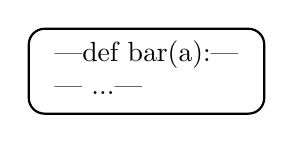
\begin{tikzpicture}
        [mystyle/.style={rounded corners=2mm, draw=black, thick}]
        \node [minimum width=20mm, minimum height=10mm, mystyle] (prog) at (0,0) {\begin{tabular}{l}
                                                                                    |def bar(a):| \\
                                                                                    |    ...|
                                                                                  \end{tabular}};
        % \node[draw=red,thick,fit=(pict),rounded corners=.55cm,inner sep=2pt]    {};
        % \matrix [column sep=7mm, row sep=5mm] {
        %     \node (se) [draw, shape=rectangle, rounded corners=.1cm] {Strong existence}; &
        %     \node (yw) [draw, shape=circle] {Y-W}; &
        %     \node (ul) [draw, shape=rectangle] {Uniqueness in law}; \\
        %     \node (d1) [draw, shape=circle] {Defn}; & &
        %     \node (d2) [draw, shape=circle] {Defn}; \\
        %     \node (we) [draw, shape=rectangle] {Weak existence}; &
        %     \node (ec) [draw, shape=circle] {E-C}; &
        %     \node (pu) [draw, shape=rectangle] {Pathwise uniqueness}; \\
        % };
        % \draw[->, thick] (se) -- (d1);
        % \draw[->, thick] (d1) -- (we);
        % \draw[->, thick] (we) -- (yw);
        % \draw[->, thick] (yw) -- (se);
        % \draw[->, thick] (se) -- (ec);
        % \draw[->, thick] (ul) -- (ec);
        % \draw[->, thick] (ec) -- (pu);
        % \draw[->, thick] (pu) -- (yw);
        % \draw[->, thick] (pu) -- (d2);
        % \draw[->, thick] (d2) -- (ul);
    \end{tikzpicture}
    \caption{The partial parse tree generated for \texttt{bar} in the example at
    \autoref{fig:bad-prog}}
    \label{fig:seq2parse-architecture}
\end{figure}
